\definecolor{reference}{RGB}{204, 240, 187}  
\definecolor{anchor}{RGB}{255, 229, 152} 

\definecolor{locality}{RGB}{248, 206, 204} 
\definecolor{detail}{RGB}{211, 225, 245} 


\newcommand{\hlreference}[1]{{\sethlcolor{reference}\hl{#1}}}
\newcommand{\hlanchor}[1]{{\sethlcolor{anchor}\hl{#1}}}
\newcommand{\hllocality}[1]{{\sethlcolor{locality}\hl{#1}}}
\newcommand{\hldetail}[1]{{\sethlcolor{detail}\hl{#1}}}
\begin{figure*}[!hbt]
\centering
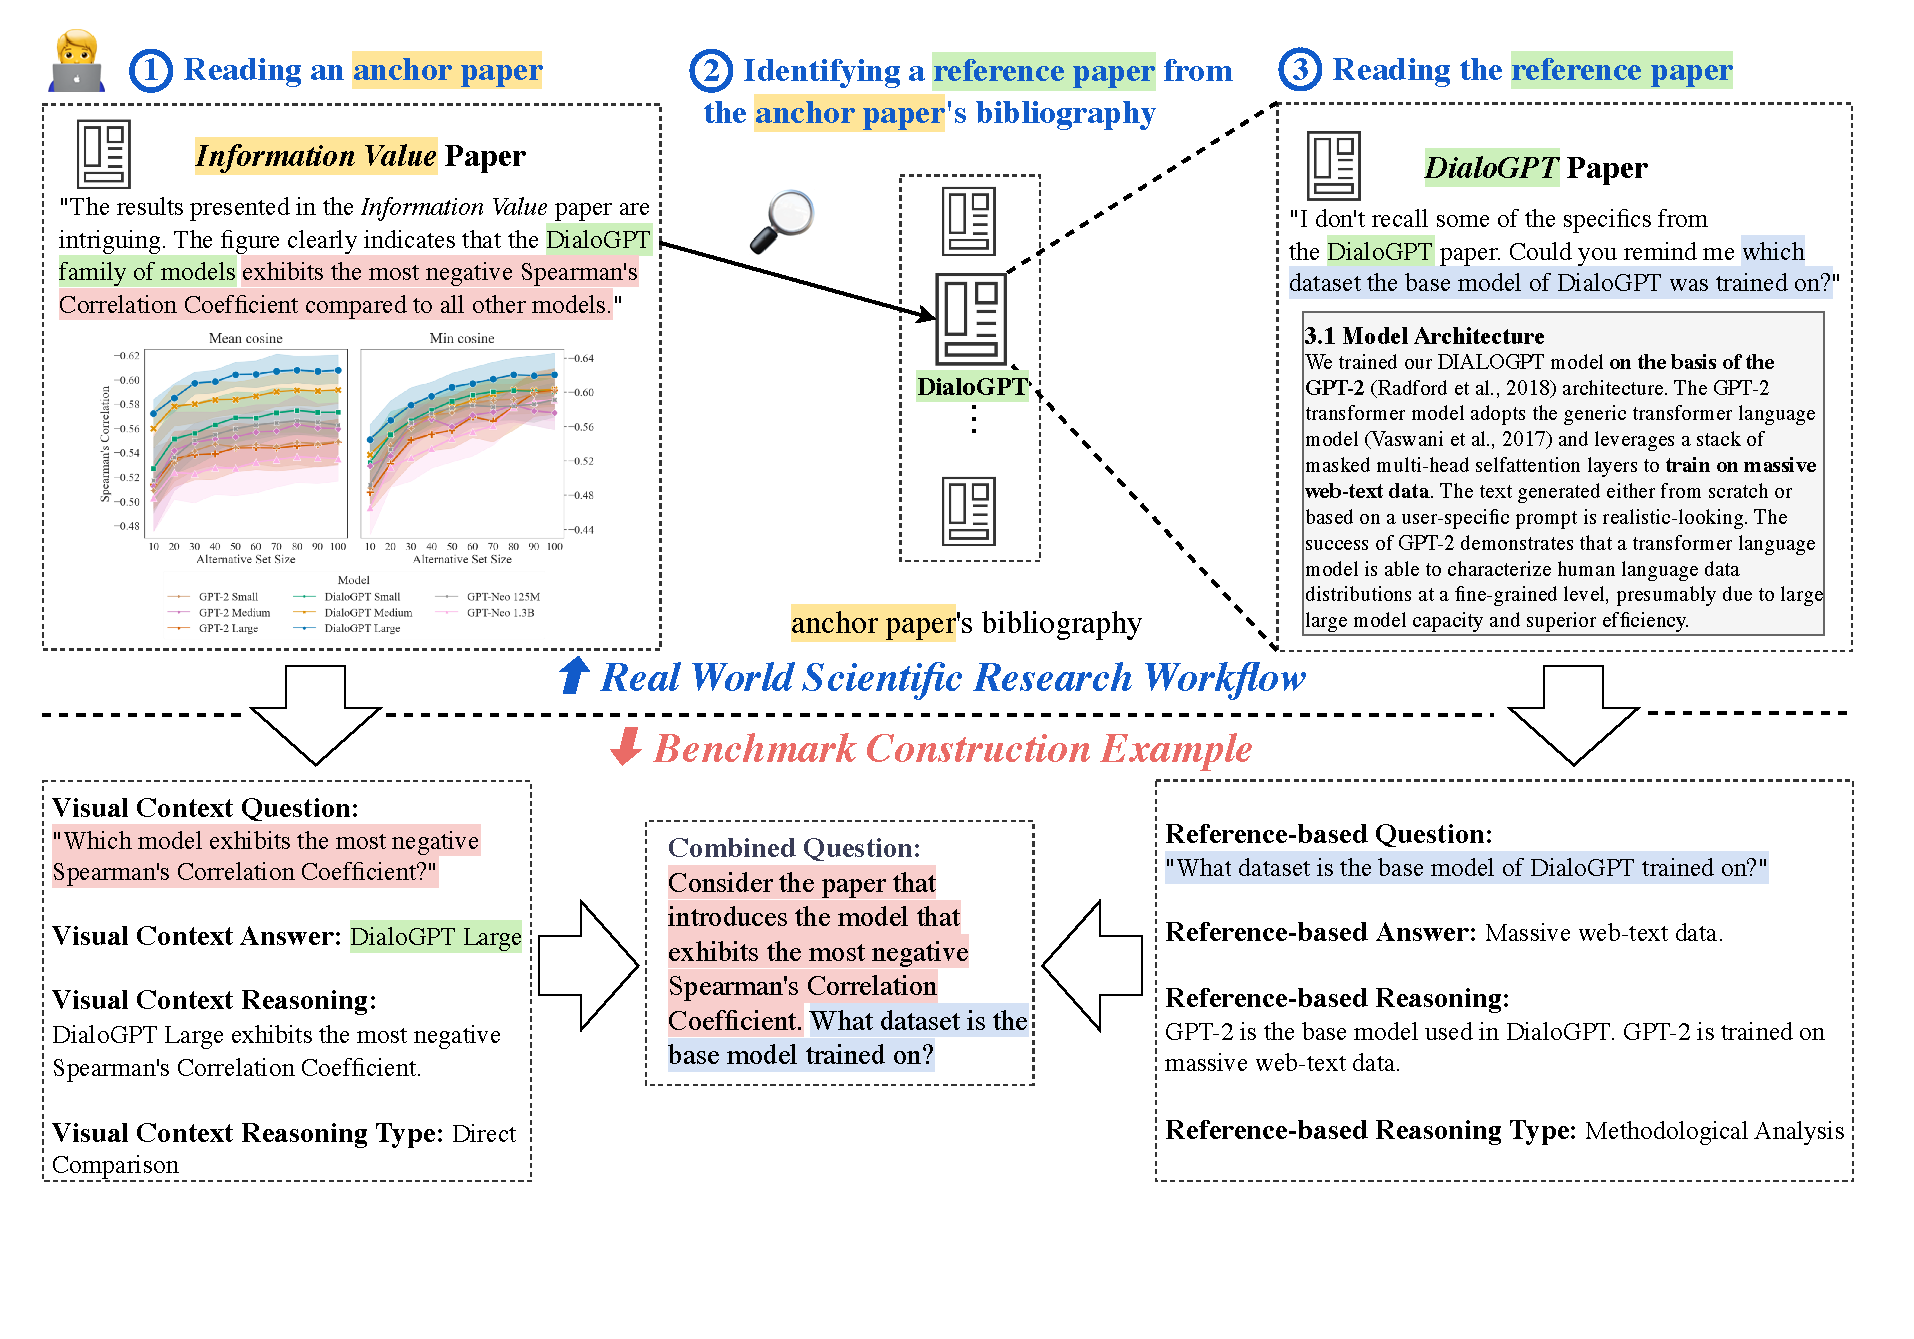
\includegraphics[width=1\textwidth]{raw_figures/figure_1.pdf}
\caption{
(\textbf{Top}) The common workflow of comparative analysis in scientific research, particularly when a result, such as a figure/table in the \hlanchor{Information Value paper (anchor paper)} \citep{giulianelli2023information}, prompts further examination of related research, such as details from \hlreference{DialoGPT (reference paper)} \citep{zhang2020dialogpt}. \textbf{(Bottom)} A demonstration of the workflow for constructing a \hllocality{visual context question}, \hldetail{reference-based question}, and combined question.
}


\label{fig:real_world}
\end{figure*}

\section{Introduction}

In scientific research, the findings presented in a paper often serve as a foundation for further investigation. When studying research papers, researchers typically explore related and cited scholarly works to acquire additional context and insights. Simultaneously, research papers are inherently multi-modal, presenting additional and often important insights in the form of figures and tables. Such properties can pose challenges for AI systems in accurately interpreting and integrating diverse data formats across multiple research papers.


Recent studies have showcased foundation models' remarkable performance across a variety of tasks in scientific literature understanding, including summarization~\citep{goyal2023news, liu2023benchmarking}, document-based question answering~\citep{newman-etal-2023-question, zhao-etal-2024-docmath, xu2024kiwi}, and scientific figure question answering~\citep{masry2022chartqa, yue2023mmmu, lu2024mathvista}.
%
However, current investigations are mostly confined to a \emph{single-document} or \emph{text-only} setting, ignoring the \emph{multi-modal} and \emph{multi-document} nature of scientific research, where insights are often derived from interpreting interconnected texts, figures, and tables across multiple scholarly works. 

To address this gap, we introduce \data, a \underline{\textbf{M}}ulti-\underline{\textbf{M}}odal, \underline{\textbf{M}}ulti-document \underline{\textbf{Sci}}entific \underline{\textbf{Q}}uestion \underline{\textbf{A}}nswering benchmark. 
%
This benchmark contains \datanum expert-annotated questions spanning 70 natural language processing (NLP) paper clusters, encompassing 3,066 papers. 
%
Each paper cluster comprises of an anchor paper and all its cited papers.
%
Inspired by the common workflow of comparative analysis in scientific research (as illustrated in Figure~\ref{fig:real_world}), our benchmark simulates a process in which a finding, derived from a \emph{scientific image} in the anchor paper, 
prompts further investigation into a specific referenced paper.
%
This simulation enriches the benchmark by requiring the models to engage in \emph{cross-referencing} among related documents, setting a new testbed for evaluating foundation models in scientific documents understanding and reasoning (Section \ref{sec:overview}). 

We evaluate a wide spectrum of \emph{open-source} and \emph{proprietary} large language models (LLMs) and large multi-modal models (LMMs). 
Our experimental results reveal significant limitations in both open-source and proprietary LMMs, particularly in their ability to translate and interpret scientific images and perform effective re-ranking based on these images, with the best-performing model, GPT-4o, achieving a Mean Reciprocal Rank (MRR) of 0.488 compared to a human expert score of 0.796, corresponding to a performance gap of 0.308. 

Similarly, we observe that both open-source and proprietary LLMs struggle with long-range retrieval tasks,
%
specifically with extracting and analyzing information from one or more academic documents. Here, the best-performing model, Command R+, achieves an accuracy score of 33.25 compared to an human expert accuracy score of 76.56\footnote{Human expert performance is assessed in the setting where the correct reference paper is known.}.
These findings underscore the challenges that current models face in handling complex, \emph{multi-modal}, \emph{multi-document}, and domain-specific information. 


Our main contributions are as follows:
\vspace{-0.5em}
\begin{itemize} [leftmargin=*]
\itemsep0em 
\item We introduce \data, a comprehensive benchmark designed to evaluate the multi-modal reasoning abilities in interpreting multiple scientific documents. 
%
\item We conduct an extensive evaluation covering a wide range of LMMs and LLMs. Our experimental results reveal a noticeable performance gap between foundation models and human experts. 
%
\item To better understand the limitations of current foundation models, we conduct a detailed analysis of scientific figure information retrieval, long-context re-ranking, and long-range retrieval, providing valuable insights for future advancements of foundation models.
\end{itemize}

